\chapter{Critical Context}

\section{Graph Terminology}
The origins of graphs theory can be traced back to Leonhard Euler and his approach to solving the Konigsberg Bridge Problem. This city was located on the Pregel River in Prussia. The river divided this city into 4 distinct areas which included an island all of which were connected by a total of 7 bridges. Euler’s representation of this problem of the individual areas as nodes and the bridges as edges is considered one of the first applications of graph theory.\cite{Dickson2006}

\begin{figure}[h]
    \centering
    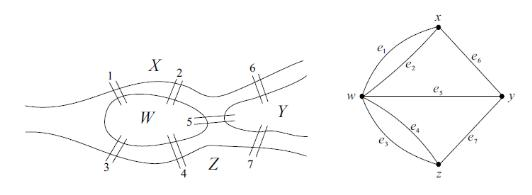
\includegraphics{euler}
    \caption{Euler’s graphical representation of the Konigsberg Bridge Problem.}
    \label{fig:Konigsberg Bridge Problem.}
\end{figure}

\\
A graph, G can be described as a triple which consists of a set of edges E (G), a set of vertices or nodes V (G) and a relationship that connects the vertices to these edges. Finite graphs are those that have V and E as a finite set. Simple graphs are those that have no loops or multiple edges. A path is simple graph in which the vertices can be ordered where two vertices can be adjacent only if they are consecutively ordered. A cycle is defined as a simple graph where the vertices can be cyclically ordered such that two vertices are adjacent only if they are consecutive in cyclical ordering. A subgraph can be thought of cycles and paths within a larger graph, where the edge relations between the subgraph and the large graph are the same. \cite{Dickson2006}\\

\section{The Limitations of traditional SNA}

In Social Network Analysis (SNA), traditionally bounded networks are considered with maybe 2 or 3 connection or link types such as friendship or advice between a node types such as people sometimes another node type such as events are also considered together. \cite{Carley2001}\\

If we consider more critically the interactions possible within our problem context of email networks we can have email networks within an organisation which are bounded and also with other organisations, clients and stakeholders and then the network does become unbounded. These networks can then be thought of as a higher order networks and as  \citeauthor{Carley2001}\cite{Carley2001} notes many tools developed for simpler networks do not scale well to increased network size and complexity and in some cases experience degradation through increased susceptibility to Type 1 and Type 2 errors. \\

The dynamics in these networks can arise from different processes depending on the context of the problem. Natural evolutionary processes would be learning, births, deaths and ageing Others could be as a result of intervention measures such removal or addition of nodes i.e. removing those who lead the system, communities forming or disintegrating. The data associated with such systems are also often incomplete and contain errors which make the process of analysis and evaluation of these systems.\cite{Carley2007}\\

Analysis approaches that go beyond traditional SNA and link analysis are therefore necessary. Within the context of such dynamic networks analysis can be performed to identify of key individuals, locating hidden groups and estimate performance.  The data analysis process on such networks then involve: \cite{Carley2001,Carley2007}

\begin{itemize}
    \item Relationship identification among nodes
    \item Network structure characterisation
    \item Locating the elite within the network
    \item Identifying points of vulnerability 
    \item Comparing networks
\end{itemize}


The approaches that enables effective analysis of such dynamic networks and help quantify their evolution over time is the motivation for this research. 

\section{Dynamic Network Analysis as an Extension to SNA}

Dynamic network analysis (DNA) aims to extend the methods, tools and techniques used in traditional Social Network Analysis (SNA) to the analysis of networks which are able to handle big dynamic multi-mode, multi-link networks with varying levels of uncertainty.  Dynamic networks also allow for probabilistic connection between nodes. \cite{Carley2001,Carley2007}\\

In \citeauthor{Carley2007}\cite{Carley2007} DNA was explored within the context of terrorism networks. Here an additional layer of complexity is added by the fact that an act of measurement changes its properties and this change propagates through the network and its state changes. Another key point is that the nodes in this network have the ability to learn. So the nodes themselves can be thought of being probabilistic compared to the more static nature of SNA nodes. \\

In a DNA representation system can be represented as relational data. This relational data structure can lend flexibility in defining multiple node types defined as multi-modal, have various types of connections among such nodes called multi-plex. The underlying attributes of both node, edges and the data change over time hence the dynamic part. \cite{Carley2007}\\

In \citeauthor{Carley2007}\cite{Carley2007} the key advances that allow for the analysis of such dynamic networks are identified as:

\begin{itemize}
    \item The meta matrix
    \item Probabilistic edges between nodes
    \item Combining social networks with cognitive science and multi-agent systems
\end{itemize}

\subsection{The Meta Matrix}
The Meta matrix is a method used in operations research and organisational management that seeks to represent the entity and class relationships as a collection of networks. In the DNA context this translates as a multimode, multiplex approach to representing systems. Therefore, the Meta matrix can contain a social network, a membership network and knowledge network and allow us to explore and analyse the connections between them. \cite{Carley2001, Carley2007, Snijders2015}

\subsection{Probabilistic Ties}

The ties or connections in the Meta matrix are probabilistic with various factors affecting their probability. This allows for inclusion of the observers’ uncertainty and the likelihood that the tie is present at the time of observation. These probabilities themselves and their temporal evolution maybe estimated by the Bayesian methods, cognitive inferencing and models of social and cognitive change. \citeauthor{Carley2001}

\subsection{Multi Agent Network Models}

As previously discussed the SNA treatment of nodes as static agents unable to learn is insufficient when dynamic networks are concerned. In DNA the nodes are able to take actions, learn from experience and alter their networks as a result. Some social and cognitive processes that influence the agent’s interactions are relative similarity, relative expertise and co-workers. The dynamic behaviour of the network emerges from these interactions and experience a shared evolution. \cite{Carley2001}\\

We briefly discuss some of the more common measures associated with networks which relate to their global and local properties. These will be important when we discuss similarity because one of the ways to assess similarity is to consider snapshots of a network attribute at different time intervals. 

\section{Network Measures}

Centrality measures are a fundamental statistic in network analysis.Two paradigms of centrality definitions are suggested. One is the means based definition of centrality or the graph theoretic and the other is the ends-based definition which is a dynamic model based view that focuses on the outcome for the nodes in a network where there is flows across the nodes . However, both approaches agree that this measure is a node level property. \cite{Borgatti2006, Borgatti2006b,Borgatti2005}\\

The network measures used in this analysis are:

\begin{itemize}
    \item Degree Centrality
    \item Closeness Centrality
    \item Betweeness Centrality
    \item Katz Centrality
    \item Load Centrality
    \item Density
    \item Average Clustering Coefficient
    \item Algebraic Connectivity
\end{itemize}

These measures are described in detail in Chapter 3, but the reason they are chosen is that the centrality measures are well understood node level properties and Density, Average Clustering Coefficient and Algebraic Connectivity are good network level properties that indicate the growth or contraction of the network as well as its communities. 


\section{Overview of Similarity Methods}

Similarity in a networks is classified as being of structural, content or keyword based. The Structural similarity or link based similarity considers the similarity of links between the nodes in the graph e.g. Cosine, Jaccard, Hub Promoted and Hub Depressed Index etc. Content similarity considers the attributes of the node in the graph. For example, on a social network this could be birth dates or hobbies of individuals. Keyword similarity aims to find similarity based on nodes representing word collections. Global Structural Similarity can be classified as being: 

\begin{itemize}
    \item Local vs. Global
    \item Parameter free vs. Parameter dependent
    \item Node Dependent vs. Path Dependent
\end{itemize}

The global structural measures aim to measure node similarity compared to the whole network. We will call them intra network similarity measures. \cite{Rawashdeh2012}\\

Inter network similarity measures are described in \cite{Dehmer2006, Koutra2011,Soundarajan2014, Zager2008, Wang2008, Zass2008,Conet2004,Bunke2000}. These
measures are classified by \citeauthor{Ashby2007}\cite{Ashby2007} into three categories:
\begin{itemize}
    \item Distance Based
    \item Feature Based
    \item Probabilistic
\end{itemize}

\subsection{Distance Based Approach}

The distance based approach is perhaps the earliest of the methods encountered which is based on edit distance \citeauthor{Bunke2000}\cite{Bunke2000}. Essentially this boils down to finding a sequence of operations such as deletion, insertion, or substitution minimising some cost function that will turn one graph into another. These involve detection and comparison of the graph isomorphism, subgraph isomorphism and maximum common subgraph detection utilising the edit distance. Although these methods are guaranteed to converge to an optimal solution their exponential complexity makes them unsuitable for large graphs.

\subsection{Feature Based Approach}

This involves calculation of a network attribute such as degree, closeness,
betweenness, and/or eigenvector centrality for the graphs and then applying a similarity measure on them that will characterise their similarity or dissimilarity. This has the benefit of being scalable to very large networks as the aggregated statistics are much smaller than the network themselves.

\subsection{Probabilistic Approach}

The methods that fall under this approach in the literature are vast. Some approaches under the probabilistic framework for graph matching are discussed here \cite{Zass2008,Yaghi2008, Spielman2007, Caetano2009}. But simply stated these methods define a probability distribution over mappings or graph embedding’s \cite{Conet2004,Caetano2009}. Graph embeddings are graphs whose nodes correspond to distinct points on a plane and the edges represents relationships connecting these points. The matching algorithm is strongly dependent upon the geometric information attached to the
graphs\cite{Conet2004,Caetano2009}. \\

Graph matching allows for recovering point correspondences. In \citeauthor{Zass2008}\cite{Zass2008} the authors show that assuming that the assignment matrix that represents these correspondences are statistically independent the high order matching problem can be represented by a Kronecker product matrix. Also they show that that a high order tensor affinity tensor can be marginalised into a one dimensional vector of probabilities. This probability vector is then updated by projection to a vector assignment space and then minimizing a distance measure (Bregman measure) \cite{Egozi2013}.

\section{Graph Similarity}

The problem of graph similarity or graph matching then becomes one of finding the equivalence of two graphs with potentially different number of nodes and edges and returning a measure within [0, 1] that captures their similarity or dissimilarity. \cite{Hanneman2005,McDiarmid2013,Ashby2007,Zass2008,Dehmer2006,Komosinski2011,Koutra2011,Rawashdeh2012,Soundarajan2014,Zager2008}\\

The key idea of graph matching in the context of dynamic networks can be summarised as finding a subgraph or an attribute that we can compare between two time instances. For example, if we consider the Degree Centrality of a network at time step 0 and then again calculate this measure at time step 1 we can apply a similarity measure on this attribute to quantify the change within the network. This can be done by means of a distance metric such as cosine similarity and others are possible. \\

The evaluation of the change in metrics over time will be done through a statistical control process. This is a concept that comes from quality engineering and it essentially involves calculating a statistic from a sequence of measurements of a random process and then comparing it so some control limit. This process translates to:

\begin{enumerate}
    \item Calculating a cumulative sum control chart which is very good for detecting small changes in mean over time
    \item Calculating a z-score for each time step $z_t = \frac{(x - \mu)}{\sigma}$
    \item Construction of two charts to detect increase and decrease in the metric
\end{enumerate}


\section{Spectral and Tensor Methods}

Spectral graph theory is the study of the eigenvectors and eigenvalues of graph matrices \cite{Spielman2007}. The spectrum of a finite graph is the spectrum of the adjacency matrix, which is the eigenvectors and eigenvalues derived from the eigendecomposition of this matrix. For an undirected graph without loops, the Laplace Matrix is the matrix indexed by a vertex set of v , with zero row sums if D is the degree matrix of a graph and A is the adjacency matrix then the Laplacian Matrix, L can be defined as $L = D – A$, where $Q = D + A$ is called the signless Laplacian Matrix of the graph. \cite{Spielman2007, Kunegis2013,Brouwer2012}\\


\citeauthor{Spielman2007}\cite{Spielman2007} note that since the eigenvalues of a graph do not depend on the vertex
ordering of the graph then they could be used to distinguish between pairs of non-isomorphic graphs. If the eigenvalues for the graphs are different then two graphs can be considered different. But he notes that this approach has problems such as the eignevectors being only determined up to sign i.e. v and –v can both be eigenvectors, so spectral embedding
comparison would result in having to check 2 K possible ways of flipping their signs. The eigenvectors can provide coordinates for each vertex in a graph which is independent of the vertex labels but for graphs for which non-trivial eigenvalues have high multiplicity the coordinate flips in addition to its rotation must also be considered. Also the coordinates denoted by the eigenvectors are not unique which means that all eigenspaces must be considered to guarantee uniqueness of the coordinates of the vertices. Hence, this approach is problematic in practice. \\

\citeauthor{Kunegis2013}\cite{Kunegis2013}, suggest that since evolution or changes in a graph over time will
lead to changes in its spectrum therefore an Eigen decomposition of the adjacency matrix can be used to characterise the this change. They then use the networks spectrum for link prediction and also discuss a method to reducing this link prediction problem to a 1D curve fitting problem. \\

\citeauthor{Duchenne2014}\cite{Duchenne2014} formulate the hypergraph matching problem as a maximization of a multilinear objective function over a tensor representing feature permutations. The tensor represents the affinity between tuples of features. A multidimensional power method is used to solve the problem and the solution is then projected onto to the closest assignment matrix. The power method utilises a tensor Eigen decomposition and is applied to point matching
using some similarity measure.

\section{Visual Methods}

More recently, the authors in \citeauthor{Behrisch2016}\cite{Behrisch2016} have proposed visualising dynamic networks and
characterising change by visualising the adjacency matrix of these networks as a matrix cube. Representing the adjacency matrix as a stack of cubes rather than node link diagrams is found to be a much more useful paradigm for analysis of dynamic networks especially when these networks are dense.\\

\citeauthor{Behrisch2016b}\cite{Behrisch2016b} have proposed Matrix Diagnostics which ranks matrix views according to the appearance of some visual patters such as lines and blocks. These are taken as a proxy for network features such as clustering. This approach has been designed to aid in the analysis, query and identification of matrices with similar patters when there are a large collection of matrices. This can also be used to judge the effectiveness of the matrix reordering methods. These methods are particularly suited to dynamic networks as it can identify most similar matrices in a graph time series by their appearance similarity. 


\section{Contributions of this study}

As we have shown from our reading of the literature that the tools applied are unprecedented in the literature and in addition to filling gaps in the current body of work we are also pushing the research in a new direction. A vast array of tools and techniques are utilised in this study. We show how aggregated centrality and assortativity measures can be used to establish a benchmark signal for a graph time series. Then we show that traditional signal processing techniques such as Fourier and Hilbert transforms can be used for the derivation of attributes. The Hilbert transform used to derive a whole range of Seismic Attributes which have intuitive explanations and are easy to understand. In addition more exotic integral transforms such as Abel and Radon can be used for dynamic network analysis and visualisation of derived attribute volumes. These transforms allow us to treat the network as a music signal and opens up the field to attributes which have no parallel in network analysis to be used from Music Information Retrieval and Digital Music analysis. \\

These measures can not only be used in aggregated in form but can be used to derive a meta attribute that can serve as a snapshot of network activity to this end we suggest RMS and NRMS measures of aggregation. Also by using correlation analysis, correlation networks, regression and manifold reduction analysis we show the relationship between these attributes. A lot of these novel attributes are fairly well correlated to existing measures while a significant number of them are not strongly correlated to any of the other metrics but from a regression perspective important in prediction of network properties such as average Degree. \\

